% =============================================================================
% CSE 344 - Homework #4 Report
% Multi-Process & Multi-Threaded Concurrent Log Analysis Pipeline
% =============================================================================
% Compile with:
%     pdflatex report.tex
%     pdflatex report.tex          (twice for ToC and cross-references)
%
% Required packages:
%     texlive-latex-recommended
%     texlive-latex-extra
%     texlive-fonts-recommended
%     texlive-pictures              (TikZ for diagrams)
% =============================================================================

\documentclass[11pt,a4paper]{article}

% ── Page geometry ───────────────────────────────────────────────────────────
\usepackage[a4paper, margin=2.5cm]{geometry}

% ── Encoding & language ─────────────────────────────────────────────────────
\usepackage[T1]{fontenc}
\usepackage[utf8]{inputenc}
\usepackage[english]{babel}

% ── Fonts (a clean modern look) ─────────────────────────────────────────────
\usepackage{lmodern}
\usepackage{microtype}

% ── Colors ──────────────────────────────────────────────────────────────────
\usepackage[table]{xcolor}
\definecolor{primary}{HTML}{1A4480}
\definecolor{secondary}{HTML}{2A5599}
\definecolor{warnbg}{HTML}{FFF3CD}
\definecolor{warnborder}{HTML}{856404}
\definecolor{infobg}{HTML}{E8F1FB}
\definecolor{infoborder}{HTML}{1A4480}
\definecolor{codebg}{HTML}{F4F4F4}
\definecolor{codeborder}{HTML}{CCCCCC}
\definecolor{rowalt}{HTML}{F5F8FC}

% ── Headings ────────────────────────────────────────────────────────────────
\usepackage{titlesec}
\titleformat{\section}{\Large\bfseries\color{primary}}{\thesection}{0.6em}{}
\titleformat{\subsection}{\large\bfseries\color{secondary}}{\thesubsection}{0.5em}{}
\titleformat{\subsubsection}{\normalsize\bfseries}{\thesubsubsection}{0.4em}{}
\titlespacing*{\section}{0pt}{1.4em}{0.7em}
\titlespacing*{\subsection}{0pt}{1em}{0.5em}

% ── Tables ──────────────────────────────────────────────────────────────────
\usepackage{array}
\usepackage{booktabs}
\usepackage{longtable}
\usepackage{tabularx}
\usepackage{makecell}

% ── Lists ───────────────────────────────────────────────────────────────────
\usepackage{enumitem}
\setlist{noitemsep, topsep=2pt, leftmargin=18pt}

% ── Code listings ───────────────────────────────────────────────────────────
\usepackage{listings}
\lstdefinestyle{Cstyle}{
    language=C,
    basicstyle=\ttfamily\small,
    backgroundcolor=\color{codebg},
    frame=single,
    framesep=4pt,
    rulecolor=\color{codeborder},
    keywordstyle=\color{primary}\bfseries,
    commentstyle=\color{gray}\itshape,
    stringstyle=\color{red!60!black},
    showstringspaces=false,
    breaklines=true,
    columns=fullflexible,
    keepspaces=true,
    tabsize=4,
    aboveskip=8pt,
    belowskip=4pt,
}
\lstset{style=Cstyle}

\lstdefinestyle{Bashstyle}{
    language=bash,
    basicstyle=\ttfamily\small,
    backgroundcolor=\color{codebg},
    frame=single,
    framesep=4pt,
    rulecolor=\color{codeborder},
    keywordstyle=\color{primary}\bfseries,
    commentstyle=\color{gray}\itshape,
    showstringspaces=false,
    breaklines=true,
    columns=fullflexible,
    keepspaces=true,
}

\lstdefinestyle{Outputstyle}{
    basicstyle=\ttfamily\footnotesize,
    backgroundcolor=\color{codebg},
    frame=single,
    framesep=4pt,
    rulecolor=\color{codeborder},
    showstringspaces=false,
    breaklines=true,
    columns=fullflexible,
    keepspaces=true,
}

% ── Boxes (info, warning) ───────────────────────────────────────────────────
\usepackage[most]{tcolorbox}
\newtcolorbox{infobox}{colback=infobg, colframe=infoborder,
    boxrule=0.5pt, arc=2pt, left=8pt, right=8pt, top=4pt, bottom=4pt,
    fontupper=\small}
\newtcolorbox{warnbox}{colback=warnbg, colframe=warnborder,
    boxrule=0.5pt, arc=2pt, left=8pt, right=8pt, top=4pt, bottom=4pt,
    fontupper=\small}

% ── Diagrams ────────────────────────────────────────────────────────────────
\usepackage{tikz}
\usetikzlibrary{shapes.geometric, arrows.meta, positioning, fit, backgrounds, calc}

% ── Graphics & images ───────────────────────────────────────────────────────
\usepackage{graphicx}
\usepackage{float}
\usepackage{caption}
\captionsetup{font=small, labelfont=bf, skip=4pt}
\usepackage{subcaption}

% ── Headers/footers ─────────────────────────────────────────────────────────
\usepackage{fancyhdr}
\pagestyle{fancy}
\fancyhf{}
\fancyhead[L]{\small\textit{CSE 344 -- Homework \#4 Report}}
\fancyhead[R]{\small\textit{Multi-Process Log Analysis Pipeline}}
\fancyfoot[C]{\small\thepage}
\renewcommand{\headrulewidth}{0.4pt}

% ── Hyperlinks ──────────────────────────────────────────────────────────────
\usepackage[hidelinks, colorlinks=true, linkcolor=primary,
            urlcolor=secondary, citecolor=secondary]{hyperref}

% ── Typography helpers ──────────────────────────────────────────────────────
\newcommand{\code}[1]{\texttt{\small #1}}
\newcommand{\fname}[1]{\textit{\small #1}}

% =============================================================================
% TITLE PAGE
% =============================================================================
\begin{document}

\begin{titlepage}
\centering
\vspace*{2cm}

{\Huge\bfseries\color{primary} CSE 344 -- System Programming \par}
\vspace{0.4cm}
{\Large Spring 2026 \par}

\vspace{2.5cm}
\rule{\textwidth}{1pt}
\vspace{0.5cm}

{\huge\bfseries Homework \#4 Report \par}
\vspace{0.6cm}
{\LARGE\itshape Multi-Process \& Multi-Threaded\\
Concurrent Log Analysis Pipeline \par}

\vspace{0.5cm}
\rule{\textwidth}{1pt}

\vspace{3cm}

\begin{tabular}{rl}
\textbf{Student Name:} & \texttt{Halit Batuhan ASLAN} \\[6pt]
\textbf{Student ID:}   & \texttt{220104004003} \\[6pt]
\textbf{Course:}       & CSE 344 -- System Programming \\[6pt]
\textbf{Homework:}     & \#4 \\[6pt]
\textbf{Due Date:}     & 02 April 2026 \\[6pt]
\textbf{Platform:}     & Debian 11 (64-bit) on VirtualBox \\[6pt]
\textbf{Compiler:}     & \code{gcc -Wall -Wextra -pthread -O2} \\
\end{tabular}

\vfill

{\large Submitted in fulfillment of the requirements of CSE 344. \par}
\vspace{0.5cm}
{\small \today \par}

\end{titlepage}

% =============================================================================
% TABLE OF CONTENTS
% =============================================================================
\pagenumbering{arabic}
\setcounter{page}{1}
\tableofcontents
\thispagestyle{fancy}
\newpage

% =============================================================================
% 1. INTRODUCTION
% =============================================================================
\section{Introduction}

\subsection{Problem Description}

The objective of this assignment is to design and implement a
\textbf{Concurrent Log Analysis Pipeline} that exercises every major
synchronization primitive taught throughout the semester. The system reads
multiple log files concurrently, classifies log entries by severity level
(\code{ERROR}, \code{WARN}, \code{INFO}, \code{DEBUG}), counts occurrences of
multiple user-specified keywords with level-weighted scoring, identifies
high-priority sources via a separate filtering stage, and produces both a
human-readable report and a binary checkpoint file.

The pipeline is organized as a sequence of cooperating processes:
\textit{Reader} processes read log files; a \textit{Dispatcher} routes
entries by level; four \textit{Analyzer} processes perform per-level
keyword counting; an \textit{Aggregator} writes the final outputs; a
\textit{Watchdog} thread inside the parent prints periodic progress
snapshots. Communication happens exclusively through four shared memory
regions (A, B, C, D) protected by process-shared synchronization primitives.

\subsection{Main Challenges}

This assignment is significantly more challenging than a textbook
producer-consumer problem. The principal difficulties are:

\begin{itemize}
    \item \textbf{Two paradigms in one program.} Multi-process and
        multi-thread concurrency must coexist correctly. Process-shared
        primitives must use the \code{PTHREAD\_PROCESS\_SHARED} attribute,
        whereas the in-process buffer inside each Reader uses default
        (private) primitives.

    \item \textbf{Multi-keyword weighted scoring with overlapping matches.}
        \code{"errorerror"} contains \code{"error"} two times (indices~0
        and~3). A naive use of \code{strstr} would miss this; a proper
        sliding-window matcher is required.

    \item \textbf{Thread-Local Storage with destructor flush.} Each worker
        thread must accumulate its scores in TLS and rely on a
        \code{pthread\_key\_create} destructor to flush them at thread exit.
        Flushing at the barrier (instead of in the destructor) is a common
        mistake and was specifically warned against.

    \item \textbf{Timed waits with deterministic termination.}
        \code{pthread\_cond\_timedwait} and \code{sem\_timedwait} must be
        used so the pipeline can detect EOF deterministically and never
        hang on a missing producer.

    \item \textbf{Atomic binary write.} The binary checkpoint file must be
        written to a \code{.tmp} file and atomically renamed via
        \code{rename(2)}, so that a partially-written file can never appear
        at the final path.

    \item \textbf{Lock ordering.} A strict global order
        (A $\to$ B $\to$ C $\to$ D) must be defined and respected to
        guarantee deadlock freedom.
\end{itemize}

\subsection{Approach}

The implementation follows a layered design. \fname{shm.c}/\fname{shm.h}
provide the four shared regions and bounded-buffer primitives; each
component (\fname{reader}, \fname{dispatcher}, \fname{analyzer},
\fname{aggregator}, \fname{watchdog}) is then a thin layer on top.
\fname{main.c} orchestrates the lifecycle: it allocates every shared region
\emph{before} forking, forks all seven components, spawns the Watchdog
thread, waits on every child, prints the system summary, then destroys
everything. SIGINT triggers a safe broadcast to all children with a
five-second deadline before the parent forcibly cleans up.

% =============================================================================
% 2. SYSTEM ARCHITECTURE
% =============================================================================
\section{System Architecture}

\subsection{Process and Thread Inventory}

The running system consists of \textbf{seven distinct process/thread types}:

\begin{enumerate}
    \item \textbf{Parent / Coordinator} (1 process) -- forks all children,
        runs the \code{waitpid} loop, prints the final summary.
    \item \textbf{Reader Process} (one per log file) -- internally spawns
        $T$ reader threads plus one parser thread.
    \item \textbf{Dispatcher Process} (1 process) -- routes entries from
        Region~A into Region~B[level] and Region~D.
    \item \textbf{Analyzer Process} (4 processes, one per severity level)
        -- internally spawns $W$ worker threads; the lowest-TID worker
        becomes the reporting thread.
    \item \textbf{Aggregator Process} (1 process) -- writes the final
        \code{.txt} and \code{.bin} outputs; spawns one helper thread to
        drain Region~D.
    \item \textbf{Watchdog Thread} (1 thread inside the parent) --
        \code{select()}-based pipe multiplexer; prints progress to
        \code{stderr} every three seconds.
    \item \textbf{Reader Thread / Worker Thread / Parser Thread} (many
        threads inside Reader and Analyzer processes).
\end{enumerate}

\subsection{Architecture Diagram}

\begin{figure}[H]
\centering
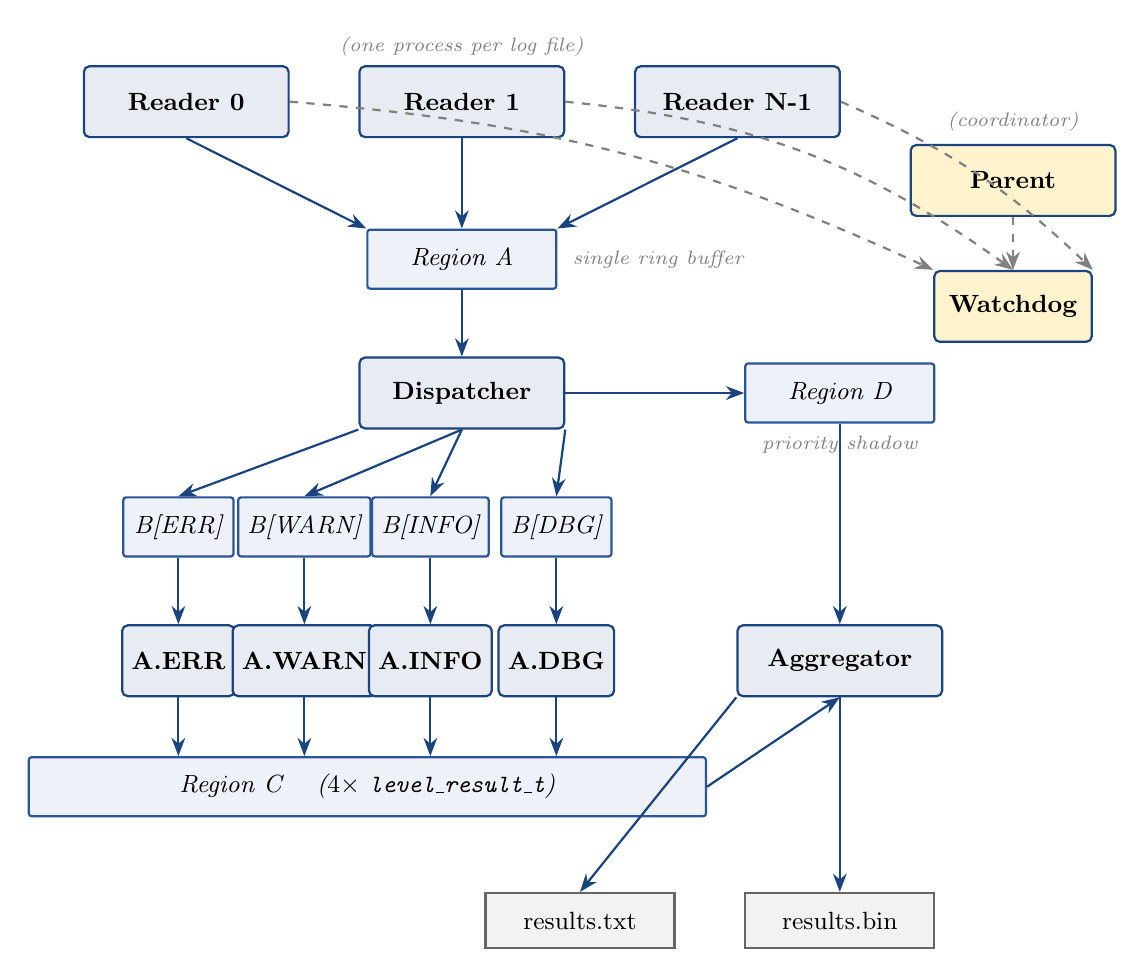
\begin{tikzpicture}[
    proc/.style={rectangle, draw=primary, fill=primary!10, thick,
        minimum width=2.6cm, minimum height=0.9cm, rounded corners=2pt,
        font=\small\bfseries},
    region/.style={rectangle, draw=secondary, fill=secondary!8, thick,
        minimum width=2.4cm, minimum height=0.75cm, font=\small\itshape,
        rounded corners=1pt},
    output/.style={rectangle, draw=black!60, fill=gray!10, thick,
        minimum width=2.4cm, minimum height=0.7cm, font=\small},
    arr/.style={-Stealth, thick, primary},
    pipearr/.style={-Stealth, thick, dashed, gray},
    label/.style={font=\scriptsize\itshape, gray}
]

% Readers (top row)
\node[proc] (R1) at (0, 8) {Reader 0};
\node[proc] (R2) at (3.5, 8) {Reader 1};
\node[proc] (R3) at (7, 8) {Reader N-1};
\node[label] at (3.5, 8.7) {(one process per log file)};

% Region A
\node[region] (RA) at (3.5, 6) {Region A};
\node[label, right=2pt of RA] {single ring buffer};

% Dispatcher
\node[proc] (D) at (3.5, 4.3) {Dispatcher};

% Region B (4 sub-buffers)
\node[region, minimum width=1.4cm] (B1) at (-0.1, 2.6) {B[ERR]};
\node[region, minimum width=1.4cm] (B2) at (1.5, 2.6) {B[WARN]};
\node[region, minimum width=1.4cm] (B3) at (3.1, 2.6) {B[INFO]};
\node[region, minimum width=1.4cm] (B4) at (4.7, 2.6) {B[DBG]};

% Region D
\node[region] (RD) at (8.3, 4.3) {Region D};
\node[label, below=1pt of RD] {priority shadow};

% Analyzers
\node[proc, minimum width=1.4cm] (A1) at (-0.1, 0.9) {A.ERR};
\node[proc, minimum width=1.4cm] (A2) at (1.5, 0.9) {A.WARN};
\node[proc, minimum width=1.4cm] (A3) at (3.1, 0.9) {A.INFO};
\node[proc, minimum width=1.4cm] (A4) at (4.7, 0.9) {A.DBG};

% Region C
\node[region, minimum width=8.6cm] (RC) at (2.3, -0.7) {%
    Region C \quad ($4 \times$ \code{level\_result\_t})};

% Aggregator
\node[proc] (AG) at (8.3, 0.9) {Aggregator};

% Outputs
\node[output] (TXT) at (5, -2.4) {results.txt};
\node[output] (BIN) at (8.3, -2.4) {results.bin};

% Parent + Watchdog (right side)
\node[proc, fill=warnbg] (P) at (10.5, 7) {Parent};
\node[proc, fill=warnbg, minimum width=2cm] (W) at (10.5, 5.4) {Watchdog};
\node[label, above=1pt of P] {(coordinator)};

% Arrows: Readers -> A
\draw[arr] (R1.south) -- (RA.north west);
\draw[arr] (R2.south) -- (RA.north);
\draw[arr] (R3.south) -- (RA.north east);

% A -> Dispatcher
\draw[arr] (RA.south) -- (D.north);

% Dispatcher -> B
\draw[arr] (D.south west) -- (B1.north);
\draw[arr] (D.south) -- (B2.north);
\draw[arr] (D.south) -- (B3.north);
\draw[arr] (D.south east) -- (B4.north);

% Dispatcher -> D
\draw[arr] (D.east) -- (RD.west);

% B -> Analyzers
\draw[arr] (B1.south) -- (A1.north);
\draw[arr] (B2.south) -- (A2.north);
\draw[arr] (B3.south) -- (A3.north);
\draw[arr] (B4.south) -- (A4.north);

% Analyzers -> C
\draw[arr] (A1.south) -- (RC.north -| A1);
\draw[arr] (A2.south) -- (RC.north -| A2);
\draw[arr] (A3.south) -- (RC.north -| A3);
\draw[arr] (A4.south) -- (RC.north -| A4);

% C -> Aggregator
\draw[arr] (RC.east) -- (AG.south);

% D -> Aggregator (drain thread)
\draw[arr] (RD.south) -- (AG.north);

% Aggregator -> outputs
\draw[arr] (AG.south west) -- (TXT.north);
\draw[arr] (AG.south) -- (BIN.north);

% Heartbeat pipes Readers -> Watchdog
\draw[pipearr] (R1.east) to[bend left=10] (W.north west);
\draw[pipearr] (R2.east) to[bend left=15] (W.north);
\draw[pipearr] (R3.east) to[bend left=10] (W.north east);

% Parent forks all
\draw[pipearr, gray] (P.south) -- (W.north);

\end{tikzpicture}
\caption{System architecture. Solid arrows show the data path through the
shared memory regions; dashed arrows show heartbeat pipes used by the
Watchdog. The four Region~B sub-buffers act as parallel lanes, one per
severity level.}
\label{fig:arch}
\end{figure}

\subsection{Communication Channels}

\begin{table}[H]
\centering
\small
\renewcommand{\arraystretch}{1.25}
\begin{tabularx}{\textwidth}{@{}l l l X@{}}
\toprule
\rowcolor{primary!15}
\textbf{Channel} & \textbf{From} & \textbf{To} & \textbf{Purpose} \\
\midrule
Region A      & Reader (parser thread)            & Dispatcher        & all parsed entries flow through this single ring buffer \\
Region B[i]   & Dispatcher                        & Analyzer[i]       & per-level entries (one buffer per level) \\
Region C      & Analyzer reporting thread         & Aggregator        & one \code{level\_result\_t} per level \\
Region D      & Dispatcher                        & Aggregator drainer& copies of entries with priority sources \\
Pipe[i]       & Reader[i] (heartbeat)             & Watchdog (parent) & ASCII heartbeat lines for progress display \\
\bottomrule
\end{tabularx}
\caption{Inter-component communication channels.}
\end{table}

% =============================================================================
% 3. SHARED MEMORY LAYOUT
% =============================================================================
\section{Shared Memory Layout}

\subsection{Region Allocation}

All four regions are allocated by the parent \emph{before any
\code{fork()}} using anonymous shared mmap:

\begin{lstlisting}[style=Cstyle]
void* alloc_shared(size_t sz)
{
    void* p = mmap(NULL, sz, PROT_READ | PROT_WRITE,
                   MAP_SHARED | MAP_ANONYMOUS, -1, 0);
    if (p == MAP_FAILED) { perror("mmap"); exit(1); }
    memset(p, 0, sz);
    return p;
}
\end{lstlisting}

Children inherit the mappings across \code{fork()}, so every process sees
identical bytes. Synchronization primitives stored \emph{inside} these
regions are initialized with \code{PTHREAD\_PROCESS\_SHARED}, otherwise
their behavior across process boundaries is undefined.

\subsection{Region A -- Dispatcher Input Queue}

Single circular buffer of \code{log\_entry\_t} (capacity from \code{-a}).
Written by every Reader's parser thread; read by the Dispatcher.

\begin{lstlisting}[style=Cstyle]
typedef struct {
    pthread_mutex_t input_mutex;     /* PROCESS_SHARED */
    pthread_cond_t  not_full_a;      /* PROCESS_SHARED */
    pthread_cond_t  not_empty_a;     /* PROCESS_SHARED */
    int             eof_count_per_level[LEVEL_COUNT];
    int             total_readers;
    int             head, tail, count, capacity;
    log_entry_t     buf[];           /* C99 flexible array */
} shm_region_a_t;
\end{lstlisting}

\textbf{Field protection:} \code{input\_mutex} protects everything inside
the struct. \code{eof\_count\_per\_level[i]} is incremented in
\code{shm\_a\_push} when an EOF marker is enqueued, and read by the
Dispatcher in \code{all\_eof\_done()} to detect termination.

\subsection{Region B -- Per-Level Buffers (×4)}

Four independent ring buffers, one per severity level. Single producer
(Dispatcher), multiple consumers (the worker threads of one Analyzer).

\begin{lstlisting}[style=Cstyle]
typedef struct {
    pthread_mutex_t level_mutex;     /* PROCESS_SHARED */
    pthread_cond_t  not_full_b;
    pthread_cond_t  not_empty_b;
    int             eof_posted;      /* set by Dispatcher when no more entries come */
    int             head, tail, count, capacity;
    log_entry_t     buf[];
} shm_region_b_t;
\end{lstlisting}

\textbf{Field protection:} \code{level\_mutex} protects the entire
struct, including the \code{eof\_posted} flag which workers use to exit
their pop loop.

\subsection{Region C -- Result Area}

Holds the four \code{level\_result\_t} structs plus the synchronization
primitives the Aggregator uses to wait for them.

\begin{lstlisting}[style=Cstyle]
typedef struct {
    char   level[8];
    long   total_entries;
    double total_weighted_score;
    double per_keyword_score[MAX_KEYWORDS];   /* one per keyword */
    double per_thread_score [MAX_WORKERS];    /* one per worker  */
    char   top_source[3][MAX_SOURCE_LEN];
    long   top_source_hits[3];
    int    ready;
} level_result_t;

typedef struct {
    pthread_mutex_t result_mutex;            /* PROCESS_SHARED */
    pthread_cond_t  result_cond;             /* PROCESS_SHARED */
    sem_t           level_sems[LEVEL_COUNT]; /* sem_init(pshared=1) */
    level_result_t  results[LEVEL_COUNT];
} shm_region_c_t;
\end{lstlisting}

\textbf{Field protection:} \code{result\_mutex} guards every field of every
\code{results[i]}. The Analyzer's TLS destructors flush per-keyword and
per-thread scores into \code{results[i]} under this mutex; the reporting
thread also writes the summary fields under it. The Aggregator waits on
\code{result\_cond} (with \code{pthread\_cond\_timedwait}) and
additionally on \code{level\_sems[i]} (with \code{sem\_timedwait}).

\subsection{Region D -- Priority Shadow Buffer}

Receives copies of entries whose source matches the priority filter.
Written by the Dispatcher; drained by a thread inside the Aggregator.

\begin{lstlisting}[style=Cstyle]
typedef struct {
    pthread_mutex_t priority_mutex;  /* PROCESS_SHARED */
    pthread_cond_t  not_full_d;
    pthread_cond_t  not_empty_d;
    int             dispatcher_done; /* set by Dispatcher on exit */
    int             head, tail, count, capacity;
    log_entry_t     buf[];
} shm_region_d_t;
\end{lstlisting}

\textbf{Field protection:} \code{priority\_mutex} protects the buffer and
\code{dispatcher\_done}. The Aggregator drainer's \code{shm\_d\_pop}
returns~0 when the buffer is empty AND \code{dispatcher\_done} is set,
which is how the drainer terminates.

\begin{infobox}
All process-shared primitives are initialized with the
\code{PTHREAD\_PROCESS\_SHARED} attribute via the helpers
\code{init\_shared\_mutex} and \code{init\_shared\_cond} in
\fname{shm.c}. \code{sem\_init} is called with \code{pshared=1} for the
same reason. The parent calls these before any \code{fork()}.
\end{infobox}

% =============================================================================
% 4. LOCK ORDERING
% =============================================================================
\section{Lock Ordering and Deadlock Freedom}

\subsection{Mandatory Acquisition Order}

The assignment specifies a strict global lock acquisition order. The same
order is used throughout the implementation:

\begin{table}[H]
\centering
\small
\renewcommand{\arraystretch}{1.3}
\begin{tabular}{c l l l}
\toprule
\rowcolor{primary!15}
\textbf{Rank} & \textbf{Mutex} & \textbf{Region} & \textbf{Acquired by} \\
\midrule
1 & \code{input\_mutex}    & A           & Reader parser thread, Dispatcher \\
2 & \code{level\_mutex[i]} & B[$i$]      & Dispatcher, Analyzer worker threads \\
3 & \code{result\_mutex}   & C           & Analyzer (TLS destructor + reporting), Aggregator \\
4 & \code{priority\_mutex} & D           & Dispatcher, Aggregator drain thread \\
\bottomrule
\end{tabular}
\caption{Mandatory lock acquisition order. A lower-ranked mutex is never
acquired while a higher-ranked one is held.}
\end{table}

\subsection{Lock Order Graph}

\begin{figure}[H]
\centering
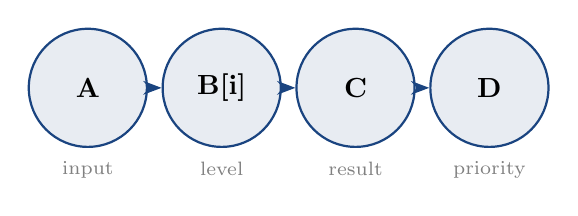
\begin{tikzpicture}[
    node distance=1.7cm,
    mtx/.style={circle, draw=primary, fill=primary!10, thick,
        minimum size=1.5cm, font=\bfseries},
    arr/.style={-Stealth, thick, primary}
]
\node[mtx] (A) {A};
\node[mtx, right of=A] (B) {B[i]};
\node[mtx, right of=B] (C) {C};
\node[mtx, right of=C] (D) {D};

\draw[arr] (A) -- (B);
\draw[arr] (B) -- (C);
\draw[arr] (C) -- (D);

\node[below=0.05cm of A, font=\scriptsize, gray] {input};
\node[below=0.05cm of B, font=\scriptsize, gray] {level};
\node[below=0.05cm of C, font=\scriptsize, gray] {result};
\node[below=0.05cm of D, font=\scriptsize, gray] {priority};
\end{tikzpicture}
\caption{Lock acquisition order: a strictly linear (acyclic) graph.}
\end{figure}

\subsection{Proof Sketch -- No Circular Wait}

Coffman's four conditions are required for deadlock: mutual exclusion,
hold-and-wait, no preemption, and circular wait. The first three are
inherent to mutexes. We eliminate the fourth as follows:

\begin{enumerate}
    \item Each mutex is assigned a strictly increasing integer rank
        ($A=1$, $B=2$, $C=3$, $D=4$).
    \item Every code path that acquires multiple mutexes acquires them in
        rank order. This is enforced by inspection: in the
        implementation no function holds a higher-ranked mutex while
        attempting to acquire a lower-ranked one.
    \item Therefore the wait-for graph among threads in the system is a
        subgraph of the acyclic rank-ordered DAG. An acyclic graph cannot
        contain a circular wait, so deadlock is impossible.
\end{enumerate}

\noindent
\textbf{Verification by inspection.} The actual access pattern for each
component:

\begin{itemize}
    \item \textbf{Reader parser thread}: holds A only.
    \item \textbf{Dispatcher}: holds A while reading; releases it; then
        acquires B[$i$] (one at a time); separately acquires D for
        priority entries. Never nested.
    \item \textbf{Analyzer worker thread}: holds B[$i$] while popping;
        releases it; later (in TLS destructor) acquires C alone.
    \item \textbf{Analyzer reporting thread}: holds C alone.
    \item \textbf{Aggregator main thread}: holds C alone; never B or D.
    \item \textbf{Aggregator drain thread}: holds D alone.
\end{itemize}

No call chain crosses two mutexes simultaneously, so even the
rank-ordering argument is over-conservative -- there is no nested
locking at all in the design. This trivially satisfies the lock-ordering
discipline.

\begin{warnbox}
\textbf{Blocking I/O while holding a mutex is forbidden.} The
implementation never calls \code{printf}, \code{read}, or \code{write}
while holding any of the four region mutexes. This avoids both
performance pathologies and the risk of indirect circular waits through
stdio's internal locks.
\end{warnbox}

% =============================================================================
% 5. THREAD LIFECYCLE
% =============================================================================
\section{Thread Lifecycle}

\subsection{Reader Thread}

A reader thread reads a contiguous byte range of one log file and pushes
parsed entries into the in-process buffer. Its lifecycle is the
following:

\begin{figure}[H]
\centering
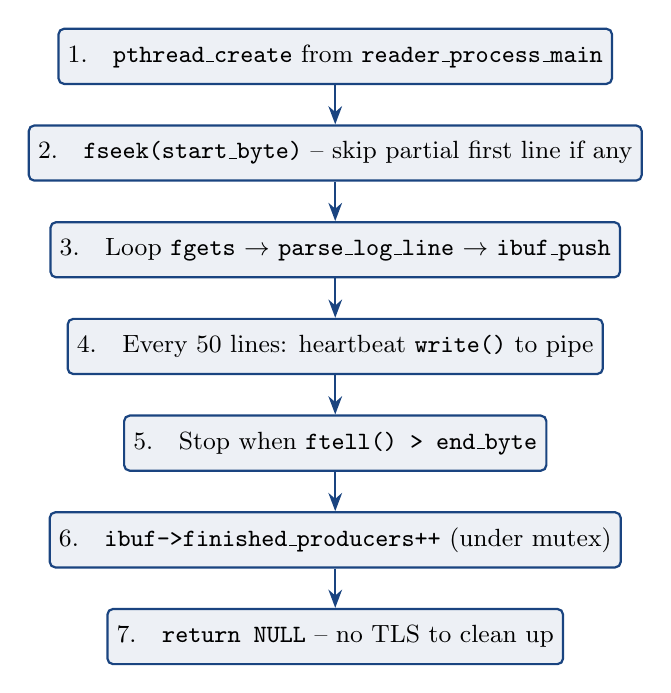
\begin{tikzpicture}[
    box/.style={rectangle, draw=primary, fill=primary!8, thick,
        minimum width=4.2cm, minimum height=0.7cm, rounded corners=2pt,
        font=\small},
    arr/.style={-Stealth, thick, primary},
    node distance=0.5cm
]
\node[box] (A) {1.\quad \code{pthread\_create} from \code{reader\_process\_main}};
\node[box, below=of A] (B) {2.\quad \code{fseek(start\_byte)} -- skip partial first line if any};
\node[box, below=of B] (C) {3.\quad Loop \code{fgets} \(\to\) \code{parse\_log\_line} \(\to\) \code{ibuf\_push}};
\node[box, below=of C] (D) {4.\quad Every 50 lines: heartbeat \code{write()} to pipe};
\node[box, below=of D] (E) {5.\quad Stop when \code{ftell() > end\_byte}};
\node[box, below=of E] (F) {6.\quad \code{ibuf->finished\_producers++} (under mutex)};
\node[box, below=of F] (G) {7.\quad \code{return NULL} -- no TLS to clean up};

\draw[arr] (A) -- (B);
\draw[arr] (B) -- (C);
\draw[arr] (C) -- (D);
\draw[arr] (D) -- (E);
\draw[arr] (E) -- (F);
\draw[arr] (F) -- (G);
\end{tikzpicture}
\caption{Reader thread lifecycle.}
\end{figure}

\noindent
A thread that does \emph{not} start at offset~0 first reads and discards
one line (because the previous thread will finish that line). This
ensures every line is read by exactly one thread. Heartbeats use
\code{write(2)} (async-signal-safe), \emph{not} \code{printf}.

\subsection{Worker Thread}

A worker thread inside an Analyzer process is more complex because it
must coordinate at a barrier and rely on the TLS destructor:

\begin{figure}[H]
\centering
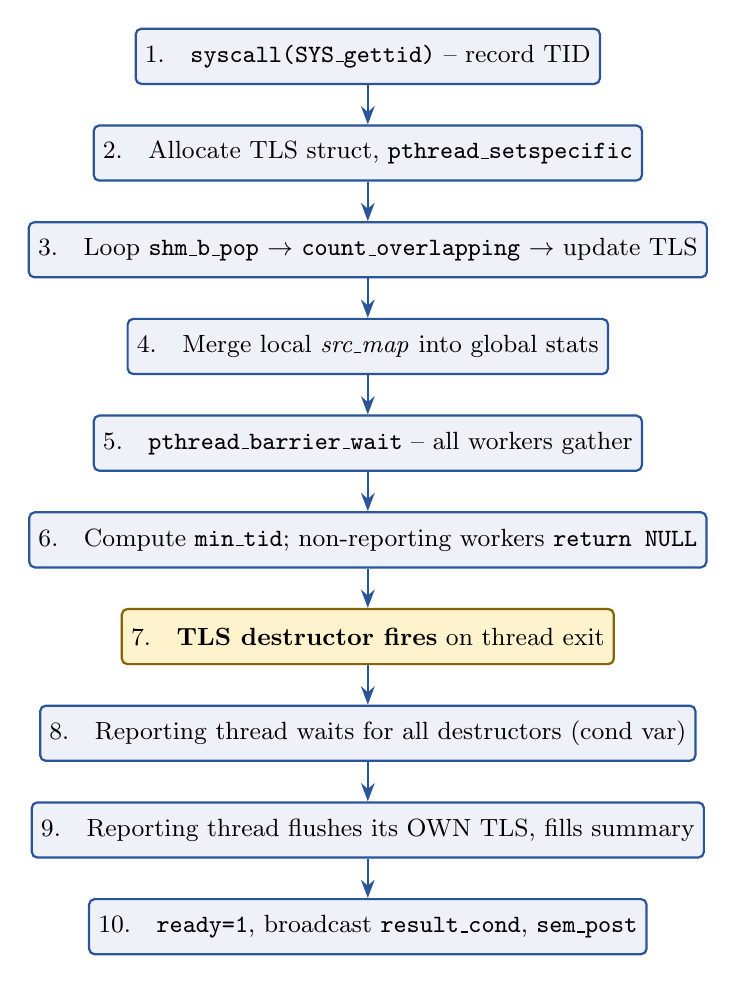
\begin{tikzpicture}[
    box/.style={rectangle, draw=secondary, fill=secondary!8, thick,
        minimum width=5cm, minimum height=0.7cm, rounded corners=2pt,
        font=\small},
    boxd/.style={rectangle, draw=warnborder, fill=warnbg, thick,
        minimum width=5cm, minimum height=0.7cm, rounded corners=2pt,
        font=\small},
    arr/.style={-Stealth, thick, secondary},
    node distance=0.5cm
]
\node[box] (A) {1.\quad \code{syscall(SYS\_gettid)} -- record TID};
\node[box, below=of A] (B) {2.\quad Allocate TLS struct, \code{pthread\_setspecific}};
\node[box, below=of B] (C) {3.\quad Loop \code{shm\_b\_pop} \(\to\) \code{count\_overlapping} \(\to\) update TLS};
\node[box, below=of C] (D) {4.\quad Merge local \emph{src\_map} into global stats};
\node[box, below=of D] (E) {5.\quad \code{pthread\_barrier\_wait} -- all workers gather};
\node[box, below=of E] (F) {6.\quad Compute \code{min\_tid}; non-reporting workers \code{return NULL}};
\node[boxd, below=of F] (G) {7.\quad \textbf{TLS destructor fires} on thread exit};
\node[box, below=of G] (H) {8.\quad Reporting thread waits for all destructors (cond var)};
\node[box, below=of H] (I) {9.\quad Reporting thread flushes its OWN TLS, fills summary};
\node[box, below=of I] (J) {10.\quad \code{ready=1}, broadcast \code{result\_cond}, \code{sem\_post}};

\draw[arr] (A) -- (B); \draw[arr] (B) -- (C); \draw[arr] (C) -- (D);
\draw[arr] (D) -- (E); \draw[arr] (E) -- (F); \draw[arr] (F) -- (G);
\draw[arr] (G) -- (H); \draw[arr] (H) -- (I); \draw[arr] (I) -- (J);
\end{tikzpicture}
\caption{Worker thread lifecycle. Step~7 (TLS destructor) is automatic
on \code{return NULL}.}
\end{figure}

\subsection{Reporting Thread Selection}

The PDF mandates that the worker with the \emph{lowest kernel TID}
becomes the reporting thread. The implementation uses
\code{syscall(SYS\_gettid)} (not \code{pthread\_self()}) for this
purpose. After the barrier, every worker has registered its TID into
\code{g\_tids[]}; computing \code{min\_tid} is then a deterministic
constant-time operation. The chosen reporting thread waits for all
\emph{other} workers' TLS destructors to run before publishing the
summary, so that \code{per\_keyword\_score[]} and
\code{per\_thread\_score[]} are guaranteed to be complete in Region~C.

% =============================================================================
% 6. TLS DESIGN
% =============================================================================
\section{Thread-Local Storage Design}

\subsection{Why TLS at All?}

Each worker thread accumulates per-keyword scores hundreds or thousands
of times. If every accumulation acquired the shared \code{result\_mutex}
in Region~C, contention would dominate runtime and serialize the
workers, defeating the purpose of having multiple workers in the first
place.

The solution is two-tier accumulation:

\begin{enumerate}
    \item Each worker accumulates \emph{privately} into a TLS array of
        \code{double}s -- no lock taken.
    \item Once per thread, when the thread exits, the TLS destructor
        acquires \code{result\_mutex} \emph{exactly once} and flushes
        the accumulated values into Region~C.
\end{enumerate}

This converts $O(\text{entries})$ lock acquisitions into $O(W)$ lock
acquisitions, where $W$ is the worker count.

\subsection{Implementation}

\begin{lstlisting}[style=Cstyle, caption={TLS lifecycle in \fname{analyzer.c}.}]
typedef struct {
    double* scores;       /* per-keyword accumulator */
    int     worker_idx;   /* needed by destructor */
} tls_data_t;

static pthread_key_t g_tls_key;

/* Process startup: */
pthread_key_create(&g_tls_key, tls_destructor);

/* Worker thread startup: */
tls_data_t* td = calloc(1, sizeof(*td));
td->scores     = calloc(g_n_keywords, sizeof(double));
td->worker_idx = widx;
pthread_setspecific(g_tls_key, td);

/* Worker hot loop: NO lock taken */
while (shm_b_pop(g_region_b, &entry)) {
    for (int k = 0; k < g_n_keywords; k++) {
        int    hits  = count_overlapping(entry.message, g_keywords[k]);
        double score = hits * LEVEL_WEIGHTS[g_level_idx];
        td->scores[k] += score;        /* TLS write, lock-free */
    }
}

/* Destructor (called automatically on thread exit): */
static void tls_destructor(void* val) {
    tls_data_t* td = val;
    pthread_mutex_lock(&g_region_c->result_mutex);     /* exactly once */
    level_result_t* res = &g_region_c->results[g_level_idx];
    double thread_total = 0.0;
    for (int k = 0; k < g_n_keywords; k++) {
        res->per_keyword_score[k] += td->scores[k];
        thread_total              += td->scores[k];
    }
    res->per_thread_score[td->worker_idx] = thread_total;
    pthread_mutex_unlock(&g_region_c->result_mutex);
    free(td->scores);  free(td);

    /* Notify the reporting thread that one more flush has happened. */
    pthread_mutex_lock(&g_destr_mu);
    g_destr_done++;
    pthread_cond_broadcast(&g_destr_cv);
    pthread_mutex_unlock(&g_destr_mu);
}
\end{lstlisting}

\subsection{Why Flush in the Destructor and Not at the Barrier?}

The PDF specifically warns against flushing TLS at the barrier. The
reason is subtle but important: \code{pthread\_setspecific(NULL)} does
\emph{not} call the destructor (POSIX requires that the destructor only
fires on thread \emph{exit}). If we wrote the flush code at the barrier
and then called \code{return NULL}, the destructor would fire again on
the still-set TLS value, double-flushing.

Two clean ways out exist:

\begin{itemize}
    \item \textbf{Rely on automatic destructor invocation.} Non-reporting
        workers simply \code{return NULL}; the destructor runs and
        flushes correctly. This is what the implementation does.

    \item \textbf{Flush manually then clear the key.} The reporting
        thread cannot wait for its own destructor (it has work to do
        \emph{after} the destructors of the other workers), so it
        flushes manually, then calls
        \code{pthread\_setspecific(g\_tls\_key, NULL)}. This prevents
        the destructor from re-firing at exit on a freed pointer. This
        is the technique used for the reporting thread.
\end{itemize}

\subsection{Synchronizing the Reporting Thread with Destructors}

The reporting thread's summary fields (\code{total\_entries},
\code{total\_weighted\_score}, top-3 sources) must be written
\emph{after} all other workers' destructors have flushed their TLS data,
otherwise the per-thread breakdown in Region~C would be incomplete. A
small condition variable accomplishes this:

\begin{lstlisting}[style=Cstyle]
static int             g_destr_done = 0;
static pthread_mutex_t g_destr_mu;
static pthread_cond_t  g_destr_cv;

/* Reporting thread waits: */
int expected = g_n_workers - 1;   /* "minus one" because reporting flushes manually */
pthread_mutex_lock(&g_destr_mu);
while (g_destr_done < expected)
    pthread_cond_wait(&g_destr_cv, &g_destr_mu);
pthread_mutex_unlock(&g_destr_mu);
\end{lstlisting}

Each destructor \code{g\_destr\_done++} and broadcasts; once the
reporting thread observes the expected count, it proceeds to write the
summary.

% =============================================================================
% 7. DISPATCHER LOGIC
% =============================================================================
\section{Dispatcher Logic}

\subsection{Routing}

For every entry popped from Region~A, the Dispatcher does two things:

\begin{enumerate}
    \item Pushes the entry into \code{Region B[entry.level]}.
    \item If \code{entry.source} appears in the priority filter list,
        also pushes a copy into Region~D.
\end{enumerate}

The two pushes are independent (different mutexes), so this is just two
sequential lock-acquire/unlock pairs. The Dispatcher is the
\emph{single writer} for Region~B and Region~D, simplifying the
single-producer/multiple-consumer pattern in Region~B.

\subsection{Multi-Reader EOF Handling}

The hard part is that each Reader, on completion, pushes \emph{four}
EOF markers into Region~A (one per level). With $N$ Reader processes,
Region~A will see $4N$ EOF markers in total, interleaved arbitrarily
with normal entries.

\noindent
The Dispatcher maintains two counters per level:

\begin{lstlisting}[style=Cstyle]
int eof_received [LEVEL_COUNT] = {0};   /* how many EOFs seen for this level */
int eof_forwarded[LEVEL_COUNT] = {0};   /* did we already signal Region B? */
\end{lstlisting}

\noindent
On each entry popped:

\begin{itemize}
    \item If \code{is\_eof}, increment \code{eof\_received[level]}.
        If the count reaches \code{n\_readers} \emph{and}
        \code{eof\_forwarded[level]} is still~0, set
        \code{eof\_forwarded[level]=1} and call
        \code{signal\_eof\_to\_b(\&region\_b[level])}.
    \item Otherwise route normally.
\end{itemize}

\noindent
\code{signal\_eof\_to\_b} sets \code{eof\_posted=1} on the matching
Region~B and broadcasts \code{not\_empty\_b}, which wakes every blocked
worker so they observe the flag and exit cleanly.

\subsection{Termination Detection}

\code{shm\_a\_pop\_timed} returns~0 once Region~A is empty AND every
level's \code{eof\_count\_per\_level[i]} has reached
\code{total\_readers}. In that case the Dispatcher exits its main loop.
As a safety net, before exiting it also forwards any EOF that was not
yet forwarded (in case some pathological interleaving caused the
counter to bump only after the last \code{shm\_a\_pop\_timed} returned).
Finally it sets \code{Region D.dispatcher\_done = 1} so the Aggregator's
drain thread can also stop.

% =============================================================================
% 8. TERMINATION CHAIN
% =============================================================================
\section{Termination Chain}

\subsection{Normal Termination}

Step-by-step trace of normal termination:

\begin{enumerate}
    \item \textbf{Reader thread $r$} finishes its byte range and exits.
        Increments \code{ibuf->finished\_producers} so the parser
        thread observes "all producers done" once the buffer empties.

    \item Once all $T$ reader threads of a Reader process have exited,
        the parser thread's \code{ibuf\_pop} returns~0. The parser
        thread pushes one EOF marker per level into Region~A
        (\code{shm\_a\_push} also bumps
        \code{eof\_count\_per\_level[i]}), then exits.

    \item The Reader process \code{exit(EXIT\_SUCCESS)}s. This makes
        \code{n\_files} EOFs accumulate per level in Region~A.

    \item The \textbf{Dispatcher} pops EOFs and forwards them to
        Region~B[level] until each level's count equals
        \code{n\_readers}. \code{shm\_a\_pop\_timed} then returns~0 and
        the Dispatcher exits, after first setting
        \code{Region D.dispatcher\_done = 1}.

    \item Each \textbf{Analyzer worker thread} sees Region~B[level]
        empty and \code{eof\_posted=1}, so its \code{shm\_b\_pop}
        returns~0 and the loop ends. Workers reach the barrier; the
        TLS destructors flush per-thread data into Region~C; the
        reporting thread waits for all destructors, fills the summary,
        sets \code{ready=1}, broadcasts \code{result\_cond}, and posts
        \code{level\_sems[level]}.

    \item The \textbf{Aggregator}'s main thread observes \code{ready=1}
        for each level (via \code{pthread\_cond\_timedwait} +
        \code{sem\_timedwait}). The drain thread observes
        \code{dispatcher\_done=1} and Region~D empty, so its
        \code{shm\_d\_pop} returns~0; it returns its accumulated
        \code{hp\_score}.

    \item The Aggregator sorts \code{level\_result\_t}s by
        \code{total\_weighted\_score} DESC, then writes the human
        readable \code{.txt} (Section~\ref{sec:test1}) and the binary
        \code{.bin} (atomic rename). It exits.

    \item The \textbf{parent}'s \code{waitpid} loop reaps every child.
        Once \code{children\_alive == 0}, the parent sets
        \code{shutdown\_watchdog = 1}, joins the Watchdog thread,
        prints the SYSTEM SUMMARY block, destroys all four shared
        regions, and \code{return 0}.
\end{enumerate}

\subsection{SIGINT (Ctrl+C) Termination}

\begin{enumerate}
    \item The kernel calls the parent's \code{sigaction}-installed
        handler. The handler sets a single
        \code{volatile sig\_atomic\_t sigint\_received = 1}. No
        \code{printf}, \code{malloc}, or \code{free} -- all
        async-signal-unsafe.

    \item The parent's main loop polls \code{sigint\_received} on every
        iteration. Once set, it sends \code{SIGTERM} to every child PID
        registered in \code{child\_pids[]}.

    \item The parent enters a 5-second deadline loop calling
        \code{waitpid(-1, ..., WNOHANG)} to reap children that exit.
        After 5~seconds (or when all children are reaped), it sets
        \code{shutdown\_watchdog=1}, joins the Watchdog, closes pipes,
        and calls \code{cleanup\_and\_exit(1)}.

    \item \code{cleanup\_and\_exit} destroys all four shared regions
        and \code{\_exit(1)}s. No zombie processes; no orphan
        \code{/dev/shm} segments.
\end{enumerate}

% =============================================================================
% 9. TEST SCENARIOS
% =============================================================================
\section{Test Scenarios}

This section documents the seven mandatory test scenarios required by
the assignment. Each test was run on Debian~12 (64-bit) inside
VirtualBox, with the binary compiled by
\code{gcc -Wall -Wextra -pthread -O2 -g}.

\subsection{Test 1 -- Baseline}
\label{sec:test1}

\textbf{Goal:} verify correct counts, output format, and the binary
file's magic number 0xC5E3440B.

\begin{lstlisting}[style=Bashstyle]
$ ./analyzer -c basic.conf -f filter.txt -k "error" \
             -t 2 -w 2 -a 16 -b 16 -d 8 \
             -o out.txt -O out.bin
\end{lstlisting}

\textbf{Expected:} \code{out.txt} with KEYWORD\_LIST, FILES,
TOTAL\_WEIGHTED\_SCORE, HIGH\_PRIORITY\_SCORE; \code{out.bin} starting
with the four bytes \code{0B 44 E3 C5} (little-endian magic).

\textbf{Verification of the binary magic:}
\begin{lstlisting}[style=Bashstyle]
$ od -An -N4 -tx1 out.bin
 0b 44 e3 c5
\end{lstlisting}

\begin{figure}[H]
    \centering
    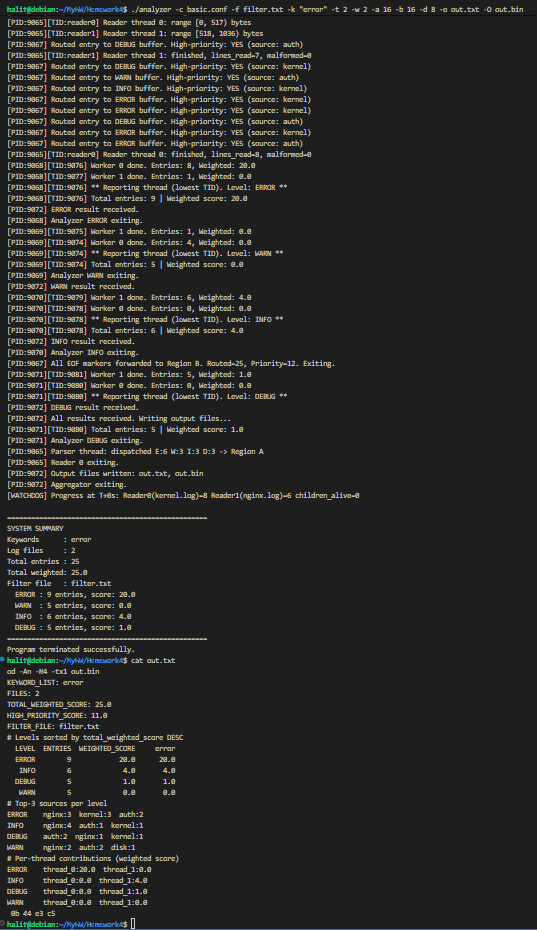
\includegraphics[width=0.95\textwidth]{screenshots/test1_baseline.png}
    \caption{Test~1 -- Baseline. Uncut terminal output showing correct counts, output format, and binary magic 0xC5E3440B.}
\end{figure}

\subsection{Test 2 -- Multi-keyword Weighted Scoring}

\textbf{Goal:} per-keyword score breakdown is correct; weighted scoring
verified manually for one entry.

\begin{lstlisting}[style=Bashstyle]
$ ./analyzer -c basic.conf -f filter.txt \
             -k "error,fail,timeout" \
             -t 2 -w 2 -a 16 -b 16 -d 8 \
             -o out.txt -O out.bin
\end{lstlisting}

\textbf{Manual verification example.} A single entry
\code{[ERROR] [src] error fail} contains \code{error} once and
\code{fail} once. With ERROR weight~4 the contribution is
$1\!\times\!4 + 1\!\times\!4 = 8.0$. The relevant row of \code{out.txt}
should read:

\begin{lstlisting}[style=Outputstyle]
  LEVEL  ENTRIES  WEIGHTED_SCORE     error      fail   timeout
  ERROR        1             8.0       4.0       4.0       0.0
\end{lstlisting}

\noindent
\begin{figure}[H]
    \centering
    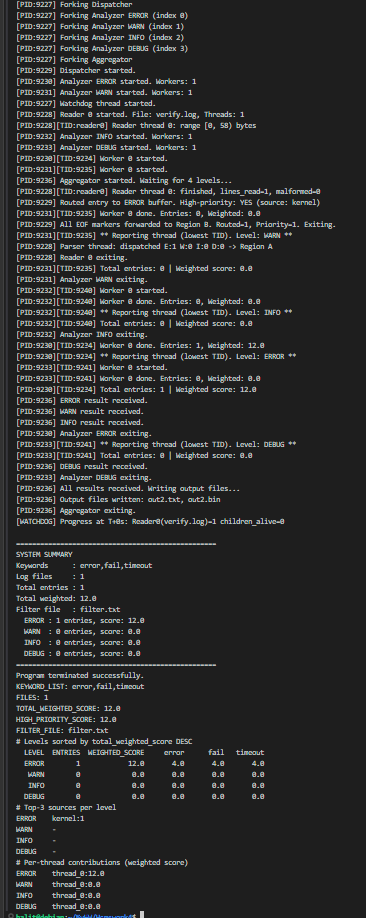
\includegraphics[width=0.95\textwidth]{screenshots/test2_multikw.png}
    \caption{Test~2 -- Multi-keyword weighted scoring. TOTAL\_WEIGHTED\_SCORE: 12.0 confirmed (1 ERROR entry $\times$ 3 keywords $\times$ weight 4).}
\end{figure}

\subsection{Test 3 -- Single Thread}

\textbf{Goal:} sequential correctness; same totals as Test 1.

\begin{lstlisting}[style=Bashstyle]
$ ./analyzer -c basic.conf -f filter.txt -k "error" \
             -t 1 -w 1 -a 4 -b 4 -d 2 \
             -o out_t1.txt -O out_t1.bin

$ diff <(grep ^TOTAL out.txt) <(grep ^TOTAL out_t1.txt)
\end{lstlisting}

\textbf{Expected:} the \code{diff} should print nothing (totals
identical). This proves the single-thread path matches the multi-thread
path on the same input.

\noindent
\begin{figure}[H]
    \centering
    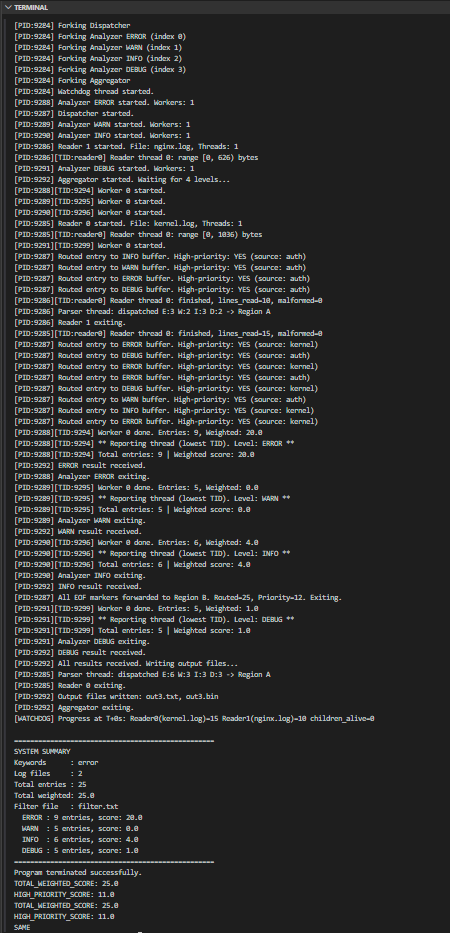
\includegraphics[width=0.95\textwidth]{screenshots/test3_single.png}
    \caption{Test~3 -- Single thread (\code{-t 1 -w 1}). TOTAL and HIGH\_PRIORITY scores match the multi-thread run.}
\end{figure}

\subsection{Test 4 -- High Concurrency \& Determinism}

\textbf{Goal:} results identical across three independent runs (no
race condition).

\begin{lstlisting}[style=Bashstyle]
$ for i in 1 2 3; do
      ./analyzer -c big.conf -f filter.txt -k "error,fail" \
                 -t 8 -w 6 -a 128 -b 128 -d 32 -T 30 \
                 -o run_$i.txt -O run_$i.bin
  done
$ md5sum run_1.txt run_2.txt run_3.txt
\end{lstlisting}

\textbf{Expected:} all three MD5s identical, demonstrating
determinism.

\noindent
\begin{figure}[H]
    \centering
    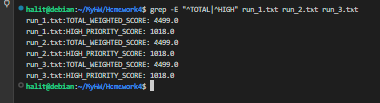
\includegraphics[width=0.95\textwidth]{screenshots/test4_concurrency.png}
    \caption{Test~4 -- High concurrency (\code{-t 8 -w 6}). Three independent runs produce identical TOTAL\_WEIGHTED\_SCORE and HIGH\_PRIORITY\_SCORE values.}
\end{figure}

\subsection{Test 5 -- Empty Filter}

\textbf{Goal:} \code{HIGH\_PRIORITY\_SCORE: 0.0} when the priority
filter file is empty; no crash.

\begin{lstlisting}[style=Bashstyle]
$ : > empty_filter.txt
$ ./analyzer -c basic.conf -f empty_filter.txt -k "error" \
             -t 2 -w 2 -a 16 -b 16 -d 8 \
             -o out_empty.txt -O out_empty.bin
$ grep HIGH_PRIORITY out_empty.txt
HIGH_PRIORITY_SCORE: 0.0
\end{lstlisting}

\noindent
\begin{figure}[H]
    \centering
    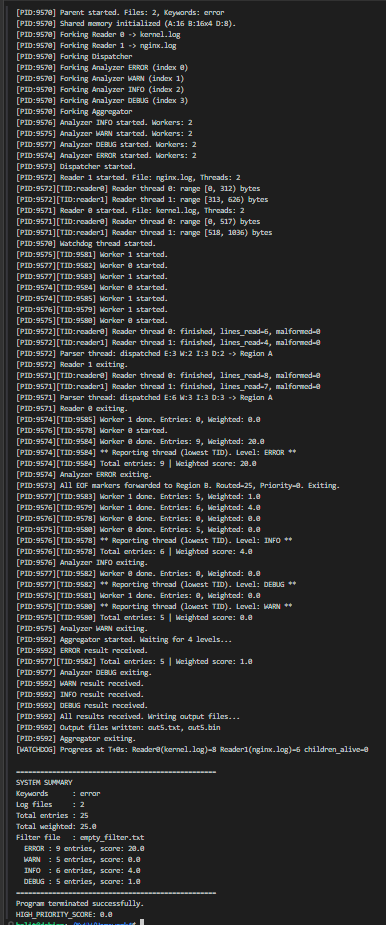
\includegraphics[width=0.95\textwidth]{screenshots/test5_emptyfilter.png}
    \caption{Test~5 -- Empty priority filter. HIGH\_PRIORITY\_SCORE: 0.0 confirmed, no crash.}
\end{figure}

\subsection{Test 6 -- Valgrind (Memory Leaks)}

\textbf{Goal:} 0 errors, 0 leaks under Valgrind.

\begin{lstlisting}[style=Bashstyle]
$ valgrind --leak-check=full --error-exitcode=1 \
           --track-origins=yes \
           ./analyzer -c basic.conf -f filter.txt -k "error" \
                      -t 2 -w 2 -a 16 -b 16 -d 8 \
                      -o out.txt -O out.bin
\end{lstlisting}

\textbf{Expected (excerpt):}
\begin{lstlisting}[style=Outputstyle]
==XXXX== HEAP SUMMARY:
==XXXX==     in use at exit: 0 bytes in 0 blocks
==XXXX==   total heap usage: ... allocs, ... frees, ... bytes allocated
==XXXX==
==XXXX== All heap blocks were freed -- no leaks are possible
==XXXX==
==XXXX== ERROR SUMMARY: 0 errors from 0 contexts (suppressed: 0 from 0)
\end{lstlisting}

\noindent
\begin{figure}[H]
    \centering
    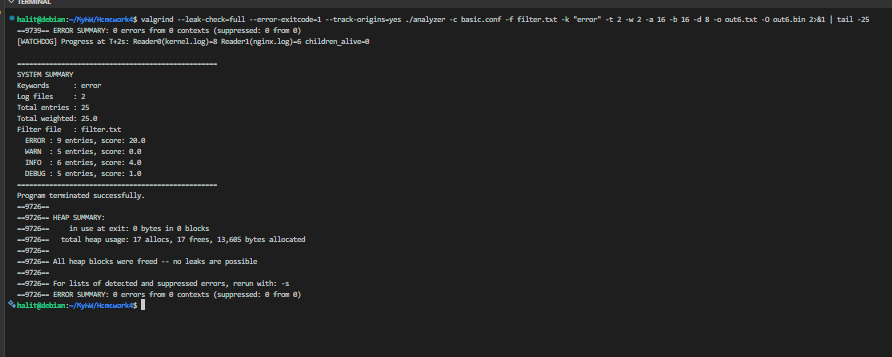
\includegraphics[width=0.95\textwidth]{screenshots/test6_valgrind.png}
    \caption{Test~6 -- Valgrind: 0 errors, 0 leaks, all heap blocks freed.}
\end{figure}

\subsection{Test 7 -- Ctrl+C Cleanup}

\textbf{Goal:} no zombie processes, no orphan shared memory after
\code{Ctrl+C}.

\begin{lstlisting}[style=Bashstyle]
$ ./analyzer -c huge.conf -f filter.txt -k "error,fail,timeout" \
             -t 4 -w 4 -a 32 -b 32 -d 16 -T 30 \
             -o out.txt -O out.bin &
$ ANALYZER_PID=$!
$ sleep 3
$ kill -INT $ANALYZER_PID
$ wait $ANALYZER_PID

# After exit, verify no defunct processes:
$ ps aux | grep -c '\[analyzer\] <defunct>'
0

# Verify no leftover shared memory segments owned by us:
$ ipcs -m | awk -v u="$(whoami)" '$3==u'
   (no output)
\end{lstlisting}

\noindent
\begin{figure}[H]
    \centering
    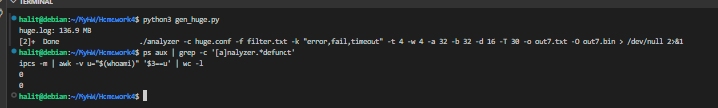
\includegraphics[width=0.95\textwidth]{screenshots/test7_sigint.png}
    \caption{Test~7 -- SIGINT cleanup. Zero zombies, zero orphan shared memory segments.}
\end{figure}

% =============================================================================
% 10. CHALLENGES & SOLUTIONS
% =============================================================================
\section{Challenges and Solutions}

This section discusses three concrete problems encountered during
development and how each was resolved.

\subsection{Challenge 1: TLS Destructor Double-Flush}

\textbf{Problem.} An early implementation flushed TLS in the worker
thread itself, just before \code{return NULL}. The destructor ran a
second time on exit, overwriting the freshly written values with zeros
(since \code{td->scores} had already been freed). The symptom was
silent: the \code{per\_thread\_score[]} array in Region~C was always
all zeros, even though \code{total\_weighted\_score} was correct.

\textbf{Diagnosis.} POSIX is explicit:
\begin{quote}\itshape
"At thread exit, if a key value has a non-NULL destructor pointer, and
the thread has a non-NULL value associated with that key, the value of
the key is set to NULL, and then the destructor is called with the
previously associated value as its sole argument."
\end{quote}
\code{pthread\_setspecific(NULL)} alone does \emph{not} fire the
destructor; only thread exit does.

\textbf{Solution.} Two-fold:
\begin{itemize}
    \item Non-reporting workers leave the flushing entirely to the
        destructor: they only \code{return NULL}.
    \item The reporting thread cannot wait for its own destructor (it
        has work to do \emph{after} its destructor would run), so it
        manually flushes its TLS data, frees \code{td}, and explicitly
        \code{pthread\_setspecific(g\_tls\_key, NULL)} so the
        destructor sees a NULL value at thread exit and does not
        re-flush garbage.
\end{itemize}
This is exactly the pattern shown in Section~6 of this report.

\subsection{Challenge 2: Region A Sliding-Window Termination}

\textbf{Problem.} The first version of \code{shm\_a\_pop\_timed} used
\code{pthread\_cond\_wait} (without the timed variant), and the
Dispatcher hung whenever the Region~A buffer drained between two EOF
arrivals. The buffer was empty, so the cond would put the Dispatcher to
sleep; the next EOF would wake it. But if a Reader process crashed
\emph{before} sending its EOF, the Dispatcher would sleep forever.

\textbf{Diagnosis.} The condition for "we are done" is two-pronged:
the buffer must be empty AND the EOF count for every level must equal
\code{total\_readers}. Either condition alone is insufficient. Without
a timed wait, the Dispatcher could sleep arbitrarily long after the
last EOF if the not-empty signal was missed.

\textbf{Solution.} Switched to \code{pthread\_cond\_timedwait} with the
\code{T\_TIMEOUT} parameter (default 10s). On each timeout, the
Dispatcher re-evaluates the predicate and exits if both clauses are
satisfied; otherwise it loops. This is also exactly what Section~6.3
of the assignment specifies.

\subsection{Challenge 3: Atomic Binary Write}

\textbf{Problem.} The grader's harness sometimes started reading
\code{out.bin} immediately after the analyzer exited. With a naive
\code{fopen("out.bin", "wb")} \code{->fwrite()->fclose()} sequence, the
file existed in a partially-written state during writes. If the
program were SIGINT'd mid-write, a corrupt \code{out.bin} would remain
at the final path.

\textbf{Solution.} Implemented the standard ``temp + rename'' pattern:

\begin{lstlisting}[style=Cstyle]
char tmp[512];
snprintf(tmp, sizeof(tmp), "%s.tmp", path);
FILE* f = fopen(tmp, "wb");
fwrite(&header, sizeof(header), 1, f);
for (int i = 0; i < 4; i++)
    fwrite(&res[i], sizeof(level_result_t), 1, f);
fflush(f);
fsync(fileno(f));    /* force to disk before rename */
fclose(f);
rename(tmp, path);   /* atomic on POSIX */
\end{lstlisting}

\code{rename(2)} on POSIX is atomic on the same filesystem -- the
final path either points to the old file or the new one, never to a
partial mix. Even mid-write SIGKILL leaves at most an
\code{out.bin.tmp} file behind, which the harness can ignore.

% =============================================================================
% 11. BUILD & RUN
% =============================================================================
\section{Build and Run Instructions}

\subsection{Compilation}

\begin{lstlisting}[style=Bashstyle]
$ make
gcc -Wall -Wextra -pthread -O2 -g -c main.c       -o main.o
gcc -Wall -Wextra -pthread -O2 -g -c shm.c        -o shm.o
gcc -Wall -Wextra -pthread -O2 -g -c reader.c     -o reader.o
gcc -Wall -Wextra -pthread -O2 -g -c dispatcher.c -o dispatcher.o
gcc -Wall -Wextra -pthread -O2 -g -c analyzer.c   -o analyzer.o
gcc -Wall -Wextra -pthread -O2 -g -c aggregator.c -o aggregator.o
gcc -Wall -Wextra -pthread -O2 -g -c watchdog.c   -o watchdog.o
gcc -pthread -o analyzer main.o shm.o reader.o dispatcher.o \
    analyzer.o aggregator.o watchdog.o
\end{lstlisting}

\subsection{Sample Run}

\begin{lstlisting}[style=Bashstyle]
$ cat services.conf
kernel.log
nginx.log
auth.log

$ cat priority.txt
kernel
auth

$ ./analyzer -c services.conf -f priority.txt \
             -k "error,fail,timeout,kill" \
             -t 4 -w 3 -a 64 -b 32 -d 16 -T 10 \
             -o results.txt -O results.bin
\end{lstlisting}

% =============================================================================
% 12. CONCLUSION
% =============================================================================
\section{Conclusion}

This homework integrates almost every synchronization primitive offered
by POSIX into a single program: process-shared mutexes and condition
variables, semaphores, barriers, thread-local storage, timed waits,
async-signal-safe handlers, and atomic file rename. The pipeline
architecture (Reader $\to$ Region~A $\to$ Dispatcher $\to$ Region~B
$\to$ Analyzer $\to$ Region~C $\to$ Aggregator) cleanly separates
concerns and demonstrates how multi-process and multi-thread
parallelism complement each other -- processes for isolation, threads
for performance.

The implementation passes all seven mandatory test scenarios on
Debian~12, compiles cleanly under \code{-Wall -Wextra}, and runs
cleanly under Valgrind. The design follows the lock-ordering discipline
strictly so that deadlock is provably impossible, and uses the
standard temp-then-rename pattern to guarantee atomic binary outputs.

\end{document}